% The code is also hosted at GitHub[1].
%
% [1] https://github.com/adityasz/cs217-lec-1

\documentclass[twoside]{article}
    \setlength{\oddsidemargin} {0.25 in}
    \setlength{\evensidemargin}{-0.25 in}
    \setlength{\topmargin}     {-0.6 in}
    \setlength{\textwidth}     {6.5 in}
    \setlength{\textheight}    {8.5 in}
    \setlength{\headsep}       {0.75 in}
    \setlength{\parindent}     {0 in}
    \setlength{\parskip}       {0.1 in}

\usepackage{amsmath}
\usepackage{amsfonts}
\usepackage{graphicx}
\usepackage{amssymb}
\usepackage{mathrsfs}   % provides \mathscr
\usepackage{physics}    % provides \norm
\usepackage{tikz}
    \usetikzlibrary{arrows.meta}
\usepackage{pgfplots}
    \pgfplotsset{compat=1.18}

%
% The following commands set up the lecnum (lecture number)
% counter and make various numbering schemes work relative
% to the lecture number.
%
\newcounter{lecnum}
\renewcommand{\thepage}    {\thelecnum-\arabic{page}}
\renewcommand{\thesection} {\thelecnum.\arabic{section}}
\renewcommand{\theequation}{\thelecnum.\arabic{equation}}
\renewcommand{\thefigure}  {\thelecnum.\arabic{figure}}
\renewcommand{\thetable}   {\thelecnum.\arabic{table}}

%
% The following macro is used to generate the header.
%
\newcommand{\lecture}[4]{
    \pagestyle{myheadings}
    \thispagestyle{plain}
    \newpage
    \setcounter{lecnum}{#1}
    \setcounter{page}{1}
    \noindent
    \begin{center}
        \framebox{
            \vbox{
                \vspace{2mm}
                \hbox to 6.28in {{\bf CS 217: Artificial Intelligence and
                                  Machine Learning \hfill Jan 10, 2024}}
                \vspace{4mm}
                \hbox to 6.28in {{\Large \hfill Lecture #1: #2  \hfill}}
                \vspace{2mm}
                \hbox to 6.28in {{\it Lecturer: #3 \hfill Scribes: #4}}
                \vspace{2mm}
            }
        }
    \end{center}
    \markboth{Lecture #1: #2}{Lecture #1: #2}

    \textbf{Disclaimer:} \textit{These notes aggregate content from several
    texts and have not been subjected to the usual scrutiny deserved by
    formal publications. If you find errors, please bring to the notice of
    the Instructor.}

    \vspace*{1mm}
}

%
% Convention for citations is authors' initials followed by the year.
% For example, to cite a paper by Leighton and Maggs you would type
% \cite{LM89}, and to cite a paper by Strassen you would type \cite{S69}.
% (To avoid bibliography problems, for now we redefine the \cite command.)
% Also commands that create a suitable format for the reference list.
%
\renewcommand{\cite}[1]{[#1]}
    \def\beginrefs{\begin{list}%
            {[\arabic{equation}]}{\usecounter{equation}
             \setlength{\leftmargin}{2.0truecm}\setlength{\labelsep}{0.4truecm}%
             \setlength{\labelwidth}{1.6truecm}}}
    \def\endrefs{\end{list}}
    \def\bibentry#1{\item[\hbox{[#1]}]}

% Use this command for a figure; it puts a figure in wherever you want it.
% usage: \fig{NUMBER}{JUST-THE-FILENAME}{CAPTION}
\newcommand{\fig}[3]{
    % \vspace{#2}
    \begin{center}
    \includegraphics{figures/#2} 
    \newline
    Figure \thelecnum.#1:~#3
    \end{center}
}
	
% Use these for theorems, lemmas, proofs, etc.
\newtheorem{theorem}{Theorem}[lecnum]
\newtheorem{lemma}[theorem]{Lemma}
\newtheorem{proposition}[theorem]{Proposition}
\newtheorem{claim}[theorem]{Claim}
\newtheorem{corollary}[theorem]{Corollary}
\newtheorem{definition}[theorem]{Definition}
\newenvironment{proof}{{\bf Proof:}}{\hfill\rule{2mm}{2mm}}

\begin{document}

\lecture{1}{The Basics of Optimization}{Swaprava Nath}{Aditya Singh, Dion Reji,
Shreyas Katdare, Brian Mackwan}

In this lecture, we discuss some basic optimization problems.

% TODO: Remove hardcoded values
\begin{center}
    \begin{tabular}{p{40 mm} | p{30 mm} | p{13 mm} | p{44 mm}}
        & Variable & Solution space & Solution complexity \\
        \hline
        Continuous optimization & take any real value (continuous) & infinite &
        polynomial in the size of the problem \\
        Discrete optimization & discrete & finite & exponential (e.g., knapsack)
    \end{tabular}
\end{center}

\section{What is optimization?}
An optimization problem involves finding the minimum value attained
by a function subject to some constraints, i.e., \[
    \min_{x \in \mathscr{C}} f(x),
\] where $f(x)$ is the objective function and $\mathscr{C}$ is the
constraint set.

\textbf{Example.} Minimize $(x - 2)^2$ with the constraint that
$x \in [0, 1] \cup [4, 7].$

Here, the objective function is $f(x) = (x - 2)^2$ and the constraint set is
$\mathscr{C} = [0, 1] \cup [4, 7].$ This is a one-variable function, and we can
easily see from the plot in figure \ref{fig:ex1} that $x^* = 1$ is the optimal
value of $x$.

\begin{figure}[b]
    \centering
    \begin{tikzpicture}[scale=1, >=latex]
        \begin{axis} [
                axis x line = bottom,
                axis y line = none,
                xlabel = $x$,
                xmin   = -5,
                xmax   = 9,
                ymin   = 0,
                ymax   = 64,
                xtick  = {0, 1, 4, ..., 7},
                ytick  = {},
                width  = 60 mm,
                height = 40 mm,
                axis line style = {<->, >={Triangle[length=2mm, width=1.5mm]}}
            ]
            \addplot [line width = 1 pt]
                expression[
                    smooth,
                    samples = 2000,
                    domain  = -5:9
                ] {(x - 2) * (x - 2)};
        \end{axis}
    \end{tikzpicture}
    \caption{A plot of $f(x) = (x - 2)^2.$}
    \label{fig:ex1}
\end{figure}

\textbf{Example.} We want to optimally place a warehouse, so that the sum of the
Euclidean distances between the warehouse and the cities is minimized.

Let the cities be located at $\mathbf{y}_1, \ldots, \mathbf{y}_m$ and the
warehouse at $\mathbf{x}$. We want to find the following: \[
    \min_{\mathbf{x} \in \mathscr{C}}
    \sum_{i = 1}^{m} \|\mathbf{x} - \mathbf{y}_i\|_2,
\] where $\mathscr{C}$ is the set of all points where we want our warehouse to
be, and $\| \cdot \|_2$ represents the $L^2$ norm, defined by \[
   \|\mathbf{x}\| := \sqrt{x_1^2 + x_2^2},
\] where $\mathbf{x} = \begin{bmatrix} x_1 \\ x_2 \end{bmatrix}$.

% Insert figure

\textbf{Example} (Image de-blurring). We consider grayscale images of size $m
\times n$, where each pixel has an intensity value in $[0, 1].$ The input image
is $\mathbf{y} = [y_{i, j}]^{m \times n}$ and the desired output is
$\mathbf{x}.$
\[
    \min_{\mathbf{x} \in [0, 1]^{m \times n}}
    \left(
        \sum_{i = 0}^{m - 1} \sum_{j = 0}^{n - 1}
            \|y_{i, j} - (k * \mathbf{x})_{i, j}\|
        + \lambda \sum_{i = 0}^{m - 1} \sum_{j = 0}^{n - 1}
            ((\mathbf{x}_{i, j} - \mathbf{x}_{i, j + 1})^2
             + (\mathbf{x}_{i + 1, j} - \mathbf{x}_{i, j})^2)
    \right)
\] Here, $\lambda$ and $k$ are the hyperparameters, which are determined by
experiment. The optimal value of $\lambda$ and $k$ depend on the image. For
example, medical images may require different $\lambda$ and $k$ as compared to
images of trees.

% Insert figure

\textbf{Example} (Machine learning; curve-fitting). We have inputs $(x_i, y_i),$
where $i \in [n].$ We want to find \[
    \min_\Theta \sum_{i = 1}^{n} \ell(h_\theta(x_i), y_i),
\] where $\ell(\cdot, \cdot)$ is a loss function, $h_\Theta(x) = w_0 + w_1 x +
w_2 x^2$ is the hypothesis (so $h_\theta(x_i)$ is the hypothesized point), and
$\Theta = (w_0, w_1, w_2)$. An example of a loss function is \[
    \ell(y_1, y_2) = (y_1 - y_2)^2.
\] 

\subsection{Linear Programming: An optimization type}
A linear program is a simple optimization type where the objective function and
constraints are given by linear relationships.

\textbf{Example} (Political Winning). Investing money to win the election

Consider a political scenario where a political party $P$ needs to invest money
to win elections. There are 3 different demographic classes, Class 1, Class 2,
and Class 3, and four issues to be addressed: A, B, C, and D. There is a
specific pattern in which people from different Classes respond to different
issues. The following table contains the number of votes gained/lost by the
political party per unit money spent, on the respective Class and issue:

\begin{table}[htbp]
  \centering
  \begin{tabular}{|c|c|c|c|}
    \hline
    \multicolumn{1}{|c|}{} & \multicolumn{3}{c|}{Classes} \\
    \hline
    Issues & Class$_1$ & Class$_2$ & Class$_3$  \\
    \hline
    $x_1 \rightarrow A $ & $-2$ & $5$ & $3$  \\
    \hline
    $x_2 \rightarrow B $ & $8$ & $2$ & $-5$  \\
    \hline
    $x_3 \rightarrow C $ & $0$ & $0$ & $10$  \\
    \hline
    $x_4 \rightarrow D $ & $10$ & $0$ & $2$ \\
    \hline
    Population & $100000$ & $200000$ & $50000$\\
    \hline
    Majority & $50000$ & $100000$ & $25000$\\
    \hline
  \end{tabular}
  \label{tab:election_grid}
\end{table}

The population of different classes along with the majority in each Class
required by the party to win the elections are also present in the table. The
aim of the political party is to minimize the total amount of money it needs to
invest, yet get the required majority across each Class. Let $x_1, x_2,x_3,x_4$
be the amount of money the party invests in issues A, B, C, and D respectively.
Hence, this problem becomes the following optimization problem:

We want to minimize $x_1+x_2+x_3+x_4$ and hence, the money spent on the election.

\begin{align}
    -2x_1 + 8x_2 +  0x_3 + 10x_4 &\geq 50000 \\
     5x_1 + 2x_2 +  0x_3 + 0x_4  &\geq 100000 \\
     3x_1 + 5x_2 + 10x_3 + 2x_4  &\geq 25000
\end{align}
Here, $x_1,x_2,x_3,x_4 \geq 0.$ Let us look at the optimal solution
$x_1^*, x_2^*, x_3^*, x_4^*.$ \[
    x_1^* = \frac{2050000}{111},\ x_2^* = \frac{425000}{111},\
    x_3^* = 0,\ x_4^* = \frac{625000}{111}.
\] 

The optimal value of
$x_1 + x_2 + x_3 + x_4 = x_1^* + x_2^* + x_3^* + x_4^* = 3100000/111.$

After multiplying and adding the equations as (1.1)$*\frac{25}{222}+$(1.2)$*\frac{46}{222}+$(1.3)$*\frac{14}{222}$, we get
\begin{equation}
        x_1+x_2+\frac{140}{222}x_3+x_4 \geq \frac{3100000}{111}
\end{equation}
$\because x_1+x_2+x_3+x_4 \geq x_1+x_2+\frac{140}{222}x_3+x_4 \geq \frac{3100000}{111}$
\\ $\therefore$ This proves that our given solution is truly the optimal solution

\subsection{Standard Form of Linear Program}
Let $\mathbf{x}$ be the vector containing variables to optimize and $\mathbf{c}$ be the vector of constants
\[
\mathbf{x} = \begin{bmatrix}
x_1 \\
x_2 \\
\vdots \\
x_n
\end{bmatrix}
\quad
\mathbf{c} = \begin{bmatrix}
c_1 \\
c_2 \\
\vdots \\
c_n
\end{bmatrix}
\]
Then we can write the standard form of linear program as follows :\\
Maximize $\mathbf{c}^T \mathbf{x}$ = $c_1x_1 + c_2x_2 + ...c_nx_n$\\
subject to constraints :
\[
\mathbf{A}_{m \times n} \mathbf{x}_{n \times 1} \leq \mathbf{b}_{m \times 1} =
\begin{bmatrix}
  b_1 \\
  b_2 \\
  \vdots \\
  b_m
\end{bmatrix}
\]
\[ \mathbf{x} \geq \mathbf{0} \]
Here $\geq$ means element wise greater than equal to i.e.\\
\[
\begin{bmatrix}
  x_1 \\
  x_2 \\
  \vdots \\
  x_n
\end{bmatrix}
\geq
\begin{bmatrix}
  0 \\
  0 \\
  \vdots \\
  0
\end{bmatrix}
\]
\[
\forall i, \quad x_i \geq 0
\]

The aforementioned problem is commonly referred to as the Primal problem, and it is accompanied by a corresponding dual problem.\\

\begin{minipage}[t]{0.45\textwidth}
  \centering
  \textbf{Primal Problem (P1)}
  \begin{align*}
    \text{maximize} \quad & \mathbf{c}^T \mathbf{x} \\
    \text{subject to} \quad & \mathbf{Ax} \leq \mathbf{b} \\
    & \mathbf{x} \geq \mathbf{0}
  \end{align*}
\end{minipage}
\hfill
\begin{minipage}[t]{0.45\textwidth}
  \centering
  \textbf{Dual Problem (P2)}
  \begin{align*}
    \text{minimize} \quad & \mathbf{b}^T \mathbf{y} \\
    \text{subject to} \quad & \mathbf{A}^T \mathbf{y} \geq \mathbf{c} \\
    & \mathbf{y} \geq \mathbf{0}
  \end{align*}
\end{minipage}

\subsection{Weak Duality Principle}

Let $\mathbf{x}$ and $\mathbf{y}$ represent feasible solutions, i.e., solutions that satisfy all the constraints, for the Primal and Dual problems, respectively then
$$\mathbf{b}^T \mathbf{y} \geq \mathbf{c}^T \mathbf{x}$$
\textbf{Proof :}
\[
\begin{aligned}
    & \mathbf{Ax} \leq \mathbf{b} \\
    & \mathbf{x}^T \mathbf{A}^T \leq \mathbf{b}^T \\
    & \text{As } \mathbf{y} \geq \mathbf{0}, \text{ multiplying it on both sides does not change the inequality} \\
    & \mathbf{x}^T \mathbf{A}^T \mathbf{y} \leq \mathbf{b}^T \mathbf{y} \\
    & \text{We know } \mathbf{A}^T \mathbf{y} \geq \mathbf{c}, \text{ so} \\
    & \mathbf{b}^T \mathbf{y} \geq \mathbf{x}^T \mathbf{c} \text{, which can also be written as } \mathbf{b}^T \mathbf{y} \geq \mathbf{c}^T \mathbf{x}.
\end{aligned}
\]
Thus weak duality principle provides relation between the solutions of Primal and Dual problems.

\subsection{Strong Duality Theorem}
If a linear programming problem
has an optimal solution, so does its dual. If $\mathbf{x^*}$ and $\mathbf{y^*}$ are the optimal solutions of Primal and Dual problems respectively then $$b^T \mathbf{y}^* = \mathbf{c}^T \mathbf{x}^*$$

\end{document}
